\documentclass[a4paper,12pt]{report}

\usepackage{cmap}
\usepackage[T2A]{fontenc}
\usepackage[utf8]{inputenc}
\usepackage[english,russian]{babel}
\usepackage{listings}
\usepackage{amsmath}
\usepackage{float}
\usepackage{csquotes}
\usepackage{mathtools}

\usepackage{xcolor}
\usepackage{hyperref}

\usepackage{graphicx}
\graphicspath{ {./images/} }

\definecolor{dkgreen}{rgb}{0,0.6,0}
\definecolor{gray}{rgb}{0.5,0.5,0.5}
\definecolor{mauve}{rgb}{0.58,0,0.82}

\lstset{
    language=Python,                 
    basicstyle=\small\sffamily, 
    numbers=left,              
    numberstyle=\tiny,          
    stepnumber=1,                   
    numbersep=5pt,                
    aboveskip=3mm,
    belowskip=3mm,
    showstringspaces=false,
    columns=flexible,
    captionpos=b, 
    basicstyle={\small\ttfamily},
    numbers=left,
    numberstyle=\tiny\color{gray},
    keywordstyle=\color{blue},
    commentstyle=\color{mauve},
    stringstyle=\color{dkgreen},
    breaklines=true,
    breakatwhitespace=true,
    tabsize=3
}

\title{Лабораторная работа №3\\Апериодические сигналы}
\author{Крынский Павел}
\date{\today}

\begin{document}

\maketitle
\tableofcontents
\listoffigures
\lstlistoflistings

\maketitle

\chapter{Упражнение 3.1}
\section{Пример утечки}

В данном упражнении нам нужно открыть \texttt{chap01.ipynb}, прочитать пояснения и  запустить примеры. Поэтому здесь я изучил все примеры с комментариями и позапускал их. \\ Также нужно заменить окно Хэмингтона одним из окон, предосталяемых NumPy и посмотреть, как они влияют на утечку. Заменим окно Хэмминга.

\begin{lstlisting}[caption=Создание других окон]
for window_func in [np.kaiser, np.bartlett]:
    wave = signal.make_wave(duration)
    if window_func.__name__ == "kaiser":
        wave.ys *= window_func(len(wave.ys) , 8)
    else:
        wave.ys *= window_func(len(wave.ys))
    spectrum = wave.make_spectrum()
    spectrum.plot(high=880)
\end{lstlisting}

\begin{figure}[H]
        \centering
        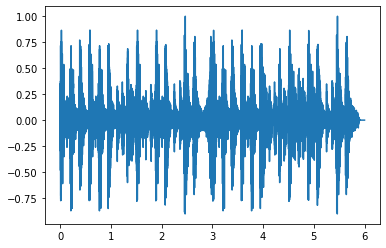
\includegraphics[width=0.75\textwidth]{1.png}
        \caption{Спектр созданных окон}
        \label{fig:lab3_fig1}
\end{figure}

Можно видеть, что окна нормально уменьшают утечку.

\chapter{Упражнение 3.2}
\section{Написание класса SawtoothChirp}

Напишем класс \texttt{SawtoothChirp}, который переопределяет \texttt{evaluate} для генерации пилообразного сигнала.

\begin{lstlisting}[caption=Класс SawtoothChirp]
class SawtoothChirp(thinkdsp.Chirp):
    def evaluate(self , ts):
        freqs = np.linspace(self.start, self.end, len(ts) - 1)
        dts = np.diff(ts)
        dphis = (2*np.pi) * freqs * dts
        phases = np.cumsum(dphis)
        phases = np.insert(phases, 0 , 0)
        frac, _ = np.modf(phases)
        ys =  self.amp * frac
        return ys
\end{lstlisting}

\section{Проверка работоспособности}

\begin{lstlisting}[caption=Проверка]
sc = SawtoothChirp(start = 200 , end = 400)
wave = sc.make_wave(duration = 1 , framerate=10000)
sp = wave.make_spectrogram(256)
sp.plot()
\end{lstlisting}
    
\begin{figure}[H]
        \centering
        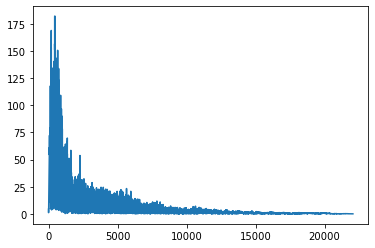
\includegraphics[width=0.75\textwidth]{2.png}
        \caption{Спекторграмма}
        \label{fig:lab3_fig2}
\end{figure}

\chapter{Упражнение 3.3}


Создаем сигнал, как просят в задании.

\begin{lstlisting}[caption=Создание сигнала]
signal = SawtoothChirp(2500 , 3000)
wave = signal.make_wave(duration = 1 , framerate = 20000)
wave.make_audio()
\end{lstlisting}

Теперь посмотрим на получившийся спектр.

\begin{lstlisting}[caption=Визуализация спектра]
cut_wave = wave.make_spectrum()
cut_wave.high_pass(10)
cut_wave.plot()
\end{lstlisting}

\begin{figure}[H]
        \centering
        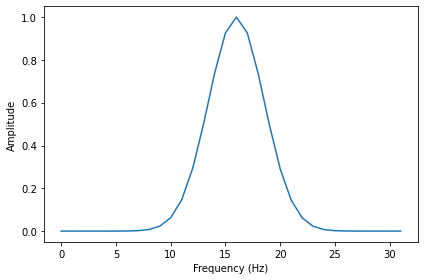
\includegraphics[width=0.75\textwidth]{3.png}
        \caption{Спектр созданного звука}
        \label{fig:lab3_fig4}
\end{figure}

\chapter{Упражнение 3.4}

Для данного задания я взял предложенный вариант файла. 

\begin{lstlisting}[caption=Загрузка]
wave = thinkdsp.read_wave('72475__rockwehrmann__glissup02.wav')
wave.make_audio()
\end{lstlisting}

Теперь рассмотрим спектрограмму.

\begin{lstlisting}[caption=Спектр]
wave.make_spectrogram(512).plot(high=5000)
\end{lstlisting}

\begin{figure}[H]
        \centering
        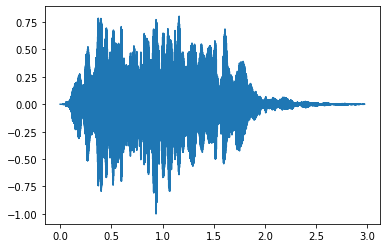
\includegraphics[width=0.75\textwidth]{4.png}
        \caption{Спектр}
        \label{fig:lab3_fig7}
\end{figure}


\chapter{Упражнение 3.5}
\section{Создание класса}

Написанный класс представляет собой тромбоноподобный сигнал с переменной частотой.

\begin{lstlisting}[caption=Создание класса]
class TromboneGliss(thinkdsp.Chirp):
    def _evaluate(self, ts):
        l1, l2 = 1.0 / self.start, 1.0 / self.end
        lengths = np.linspace(l1, l2, len(ts)-1)
        freqs = 1 / lengths
        return self._evaluate(ts, freqs)
\end{lstlisting}

\section{Создание звука и его спектрограмма}

Создадим первую часть звука от C3 до F3, где C3 - 262 Гц, а F3 - 349 Гц.

\begin{lstlisting}[caption=Создание первой части звука]
class TromboneGliss(thinkdsp.Chirp):
    def _evaluate(self, ts):
        l1, l2 = 1.0 / self.start, 1.0 / self.end
        lengths = np.linspace(l1, l2, len(ts) - 1)
        freqs = 1 / lengths
        return self._evaluate(ts,freqs)
        
signal = TromboneGliss(262,349)
waves = signal.make_wave(duration=1)
waves.apodize()
waves.make_audio()
\end{lstlisting}

Теперь создадим вторую часть звука от F3 до C3.

\begin{lstlisting}[caption=Создание второй части звука]
signal = TromboneGliss(349,262)
waves2 = signal.make_wave(duration=1)
waves2.apodize()
waves2.make_audio()
\end{lstlisting}

Затем соединим обе части в один полноценный звук.

\begin{lstlisting}[caption=Соединение двух частей звука]
wave = waves | waves2
wave.make_audio()
\end{lstlisting}

Теперь сделаем спектрограмму и расммотрим её.

\begin{lstlisting}[caption=Спектрограмма звука]
sp = wave.make_spectrogram(1024)
sp.plot(high=1000)
\end{lstlisting}

\begin{figure}[H]
        \centering
        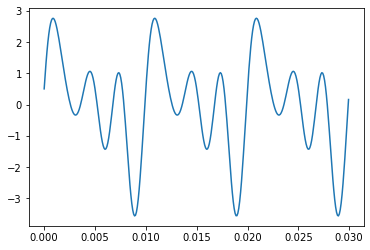
\includegraphics[width=0.75\textwidth]{5.png}
        \caption{Спектрограмма глиссандо на трамбоне}
        \label{fig:lab3_fig8}
\end{figure}


\chapter{Упражнение 3.6}

В интернете я нашёл звуки гласных.

\begin{lstlisting}[caption=Загрузка и прослушивание звука]
wave = thinkdsp.read_wave('87778__marcgascon7__vocals.wav')
wave.make_audio()
\end{lstlisting}

Посмотрим на них.

\begin{lstlisting}[caption=Участок]
sg = wave.segment(start = 0 , duration = 7)
sg.plot()
\end{lstlisting}

\begin{figure}[H]
        \centering
        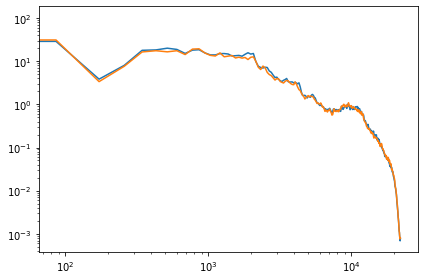
\includegraphics[width=0.75\textwidth]{6.png}
        \caption{Участок}
        \label{fig:lab3_fig9}
\end{figure}


\begin{lstlisting}[caption=Спектограмма]
wave.make_spectrogram(1024).plot(high=1000)
\end{lstlisting}

\begin{figure}[H]
        \centering
        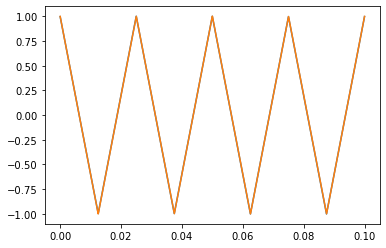
\includegraphics[width=0.75\textwidth]{7.png}
        \caption{Спектограмма}
        \label{fig:lab3_fig10}
\end{figure}

Нам важно то, что некоторые из участков темнее, а некоторые светлее (в рамках одного столбца), что соответствует спектрам соответствующих гласных.


\chapter{Выводы}

Во время выполнения лабораторной работы получены навыки работы с апериодическими сигналами, частотные компоненты которых изменяются во времени, то есть практически все звуковые сигналы. Также рассмотрены спектрограммы - распространённый способ визуализации апериодических сигналов.

\end{document}